\documentclass[11pt,a4paper]{article}
\usepackage[utf8]{inputenc}
\usepackage[T1]{fontenc}
\usepackage[italian]{babel}
\usepackage[margin=2.3cm]{geometry}
\usepackage{graphicx,booktabs,amsmath,array}
\usepackage[hidelinks]{hyperref}
\usepackage{helvet}
\renewcommand{\familydefault}{\sfdefault}
\setlength{\parskip}{4pt}
\setlength{\parindent}{0pt}

% Measured notebook times (seconds), filled from notebook_timing.R.
\newcommand{\nbTenFifty}{51}
\newcommand{\nbTenTwenty}{24}
\newcommand{\nbHundredFifty}{4\,520}
\newcommand{\nbHundredFiftyMin}{75}
\newcommand{\nbHundredFrontier}{72}
\newcommand{\nbHundredTwenty}{circa 29 minuti}

\title{Stabilit\`a dell'asset allocation nel tempo\\
\large Tredici run mensili, ottobre 2025 -- ottobre 2026, rendimenti giornalieri e settimanali,\\ con 10\,000 e con 100\,000 scenari}
\author{Progetto \texttt{portfolio-optimization-r}}
\date{2 novembre 2026}

\begin{document}
\maketitle

\section*{Sintesi}

Il tool \`e stato rieseguito a tredici date di fine mese, dal 31 ottobre 2025 al 30 ottobre 2026, ogni volta con tutta la storia disponibile fino a quella data, prima con rendimenti giornalieri e poi con rendimenti settimanali. L'esperimento \`e stato fatto due volte: con 10\,000 scenari bootstrap per run, il valore di default del tool, e con 100\,000. Per distinguere i cambiamenti dovuti ai dati da quelli dovuti al caso, alla prima e all'ultima data il bootstrap \`e stato ripetuto con sei seed diversi, a entrambi i livelli. I risultati principali sono quelli a 100\,000 scenari; quelli a 10\,000 servono a misurare cosa il rumore Monte Carlo nasconde e cosa inventa, e cosa costa toglierlo.

\begin{itemize}
\item \textbf{Le metriche di portafoglio sono stabili, a entrambi i livelli.} Con 100\,000 scenari l'ES del portafoglio Min-ES si muove in un intervallo di 0,05 punti percentuali nell'anno, lo stesso che si ottiene cambiando solo il seed. Il rapporto rendimento/ES del Max-ratio oscilla di 0,015--0,016 contro 0,005--0,009 di rumore: il movimento residuo ha una struttura leggibile (massimo a febbraio 2026, minimo a marzo, recupero fino a giugno) ed \`e spiegato dai dati.
\item \textbf{I pesi sono stabili solo con 100\,000 scenari.} A 10\,000 i pesi del Min-ES giornaliero oscillano di 6--12 punti e la ripartizione Govt/IG del Max-ratio di 15--25, ma altrettanto oscillano cambiando seed: quel movimento \`e rumore nella valle piatta dell'ES fra Euro Govt ed Euro Corp IG (4 centesimi di punto fra 20\,\% e 50\,\% di Govt). A 100\,000 scenari ogni peso del Min-ES si muove di 1,5--3,6 punti nell'anno, contro 0,5--3,5 di rumore, e la ripartizione Govt/IG del Max-ratio \`e determinata entro 4--8 punti. Il costo di usare i pesi del mese precedente non supera 0,004 punti di ES.
\item \textbf{Un cambiamento \`e genuino:} nel Max-ratio il peso azionario sale da 31,5\,\% a 39\,\% (giornaliero) e da 29,5\,\% a 39,5\,\% (settimanale), con rumore di 4 punti, a spese dei governativi (da 49\,\% a 41\,\% e da 40\,\% a 35\,\%); l'ES del portafoglio sale di conseguenza da 5,5\,\% a 6,3\,\% e da 5,7\,\% a 6,9\,\%. Lo spiegano i dati dell'anno: rendimento atteso dell'azionario in aumento e rendimento atteso dei governativi in calo, con tre mesi negativi per i governativi (marzo, luglio, settembre 2026). Questo cambiamento era visibile anche a 10\,000 scenari.
\item \textbf{Due eventi lasciano un'impronta visibile:} la correzione di marzo 2026 (azionario $-7{,}7\,\%$, tutti e quattro gli asset negativi) abbassa il rapporto del Max-ratio di 0,015--0,016 in un mese, tre volte il rumore; settembre 2026 (ancora tutti negativi, governativi $-2{,}1\,\%$) porta il rendimento atteso del Min-ES al minimo dell'anno e l'ES del Max-ratio al massimo.
\item \textbf{Giornaliero e settimanale raccontano la stessa storia con pesi diversi.} Con i rendimenti settimanali l'IG risulta meno rischioso e l'HY pi\`u rischioso e meno diversificante (effetto dell'autocorrelazione intra-settimanale e delle chiusure asincrone), quindi il Min-ES settimanale \`e sempre 73--76\,\% IG senza HY n\'e azioni, mentre quello giornaliero tiene 11--14\,\% di HY.
\item \textbf{Costo di calcolo.} Ogni portafoglio ottimo \`e la soluzione di un LP (\emph{linear program}, programma lineare: il problema di ottimizzazione in cui l'ES, grazie alla formulazione di Rockafellar e Uryasev, diventa una funzione lineare dei pesi e di una variabile ausiliaria per scenario). Il tempo di un LP cresce quasi col quadrato del numero di scenari: da 0,6--0,8 secondi a 10\,000 a 52--68 secondi a 100\,000. Lo studio (92 LP) \`e passato da 66 secondi a 94 minuti; il notebook completo, misurato, da \nbTenFifty{} secondi a \nbHundredFiftyMin{} minuti, di cui 72 nei 50 LP della frontiera. Il rumore sulle grandezze ben determinate si \`e ridotto di 2,5--5 volte, in linea con la radice di dieci; la posizione del Max-ratio lungo la frontiera (ES, peso azionario) resta invece rumorosa di 0,4--0,5 punti di ES e 4 punti di peso. \textbf{Decisione presa a valle dello studio:} il default del tool resta 10\,000 scenari, e i punti di frontiera passano da 50 a 20 (notebook da \nbTenFifty{} a \nbTenTwenty{} secondi).
\end{itemize}

\section{Metodo}

\paragraph{Dati.} Prezzi aggiustati di Yahoo Finance dalla cache del repository scaricata il 2 novembre 2026: EUNH.DE (Euro Govt), EUN5.DE (Euro Corp IG), EUNW.DE (Euro Corp HY), EXSA.DE (Europe Equity), campione comune dal 15 dicembre 2010 al 30 ottobre 2026, 4\,030 rendimenti giornalieri. Si usa un'unica serie, troncata a ogni data di analisi: ci\`o che il tool avrebbe visto a quella data, salvo le piccole revisioni retroattive che Yahoo applica alle serie aggiustate.

\paragraph{Date.} Ultimo giorno di borsa di ogni mese da ottobre 2025 a ottobre 2026: tredici run. Il campione passa da 3\,778 a 4\,030 rendimenti giornalieri (da 775 a 827 settimanali); ogni mese aggiunge 19--23 giorni, circa lo 0,5\,\% del campione.

\paragraph{Ottimizzazione.} Il tool calcola ogni portafoglio ottimo risolvendo un programma lineare (LP). L'ES non \`e lineare nei pesi, perch\'e quali scenari siano ``i peggiori'' dipende dai pesi stessi; Rockafellar e Uryasev (2000) mostrano che, aggiungendo una variabile per la soglia (il VaR) e una variabile ausiliaria per ogni scenario, pari all'eccedenza della perdita sulla soglia, minimizzare l'ES diventa un problema lineare: le incognite sono i quattro pesi, la soglia e $N$ variabili ausiliarie, i vincoli sono la somma dei pesi, i limiti per asset e un vincolo per scenario. Il Min-ES \`e questo problema; il Max-ratio lo stesso con una normalizzazione in pi\`u (Charnes e Cooper); ogni punto della frontiera \`e il Min-ES con un vincolo aggiuntivo sul rendimento atteso. Li risolve HiGHS, tramite il pacchetto R \texttt{highs}, in modo esatto. La taglia del problema cresce con $N$: \`e la ragione dei tempi della sezione~\ref{sec:perf}.

\paragraph{Pipeline.} Per ogni data e frequenza: aggregazione (identit\`a per il giornaliero, somma per settimana ISO per il settimanale), bootstrap di $N$ scenari su 60 giorni di borsa (12 settimane nel caso settimanale), ES al 95\,\%, portafoglio Min-ES e portafoglio Max-ratio con i vincoli di default (ogni asset fra 0 e 100\,\%, nessuna leva, tasso privo di rischio zero). Tutti gli altri parametri sono quelli di \texttt{R/params.R}, seed 42; $N$ vale 10\,000 nel primo esperimento e 100\,000 nel secondo, passato da riga di comando. \textbf{La frontiera e la nuvola casuale non sono state ricalcolate:} sono illustrative e non entrano nelle metriche, quindi ogni run dello studio costa una simulazione e due LP, contro i 2 + 50 LP del notebook. Questo spiega perch\'e 46 run a 100\,000 scenari (sezione~\ref{sec:perf}) costano il doppio di un solo run del notebook.

\paragraph{Misura del rumore.} Con lo stesso seed, un campione pi\`u lungo di un mese produce estrazioni diverse, quindi la differenza fra due run consecutivi mescola l'effetto dei dati nuovi e quello di un nuovo sorteggio. Per avere un metro, alla prima e all'ultima data i run sono stati ripetuti con i seed 1, 2, 3, 4, 5 e 42 a dati fissi: l'escursione fra i sei run \`e il rumore Monte Carlo puro. Un cambiamento mensile \`e considerato ``maggiore'' se supera chiaramente questa escursione. L'escursione di sei estrazioni \`e a sua volta una stima grossolana (pu\`o variare di un terzo da un gruppo di seed all'altro), quindi i confronti vanno letti come ordini di grandezza.

\paragraph{Valutazione incrociata.} I pesi ottimi di ogni mese sono stati valutati sugli scenari del mese successivo e su quelli finali, confrontando ES e rapporto con l'ottimo di quegli scenari: \`e il costo di non aggiornare l'allocazione.

\paragraph{Prestazioni.} \texttt{benchmark.R} misura, a dati fissi (ottobre 2026, giornaliero), il tempo di simulazione, dei due LP e di un punto di frontiera a 10\,000, 25\,000, 50\,000 e 100\,000 scenari, due ripetizioni ciascuno; la tabella riporta il minimo delle due, perch\'e la prima misura a 10\,000 include il riscaldamento di R e di HiGHS (2,6 secondi contro 0,6). \texttt{notebook\_timing.R} esegue invece gli stessi passi del notebook (dati, simulazione, nuvola casuale, due LP, frontiera, grafici, distribuzioni) cronometrandoli uno per uno, con numero di scenari e punti di frontiera a scelta.

\paragraph{Riproducibilit\`a.} Script \texttt{stability\_runs.R} con argomento 10000 (66 secondi) o 100000 (94 minuti), risultati in \texttt{out\_10k/} e \texttt{out\_100k/}; \texttt{benchmark.R}; \texttt{notebook\_timing.R}; tabelle e figure da \texttt{make\_tables.py} e \texttt{make\_figures.py} con argomento \texttt{10k} o \texttt{100k}; tutto nella cartella \texttt{stability/} del progetto.

\section{Risultati in sintesi}

Le tabelle~\ref{tab:summary} e~\ref{tab:summary_10k} confrontano, per ogni grandezza, l'escursione nei tredici run con quella dovuta al solo seed, a 100\,000 e a 10\,000 scenari. Le figure~\ref{fig:weights} e~\ref{fig:weights_10k} mostrano i pesi mensili ai due livelli, con il rumore sovrapposto; la figura~\ref{fig:metrics} le metriche a 100\,000. Le tabelle di dettaglio (run mensili, seed, valutazione incrociata, cosa ha aggiunto ogni mese, correlazioni, statistiche degli asset) sono quelle a 100\,000 scenari.

\begin{table}[htbp]\centering\small\setlength{\tabcolsep}{3.5pt}
\caption{Escursione delle metriche e dei pesi nei 13 run mensili, a confronto con l'escursione dovuta al solo seed Monte Carlo (6 seed, stessi dati) alla prima (ott 2025) e all'ultima data (ott 2026). Metriche in \%, pesi in punti percentuali. Run con 100\,000 scenari.}\label{tab:summary}
\begin{tabular}{lrrrrr}\toprule
grandezza & min & max & escursione & seed ott 2025 & seed ott 2026 \\\midrule
\multicolumn{6}{l}{\emph{Rendimenti giornaliero}} \\
Min-ES: ES 95\,\% & 3.90 & 3.95 & 0.05 & 0.07 & 0.05 \\
Min-ES: E[R] & 0.42 & 0.49 & 0.07 & 0.02 & 0.03 \\
Max-ratio: rapporto & 0.165 & 0.180 & 0.015 & 0.005 & 0.005 \\
Max-ratio: ES 95\,\% & 5.54 & 6.35 & 0.81 & 0.37 & 0.51 \\
Max-ratio: E[R] & 0.94 & 1.07 & 0.14 & 0.05 & 0.06 \\
Min-ES: peso Govt & 41.1 & 44.4 & 3.3 & 2.2 & 1.8 \\
Min-ES: peso IG & 43.0 & 45.8 & 2.8 & 3.5 & 2.6 \\
Min-ES: peso HY & 10.7 & 14.3 & 3.6 & 1.4 & 2.3 \\
Min-ES: peso Equity & 0.1 & 1.6 & 1.5 & 0.5 & 0.8 \\
Max-ratio: peso Govt & 40.1 & 52.2 & 12.2 & 5.2 & 4.2 \\
Max-ratio: peso IG & 14.1 & 20.3 & 6.2 & 7.6 & 6.1 \\
Max-ratio: peso HY & 0.0 & 0.0 & 0.0 & 0.7 & 0.0 \\
Max-ratio: peso Equity & 31.5 & 39.6 & 8.1 & 3.5 & 3.9 \\
\multicolumn{6}{l}{\emph{Rendimenti settimanale}} \\
Min-ES: ES 95\,\% & 3.74 & 3.79 & 0.05 & 0.08 & 0.03 \\
Min-ES: E[R] & 0.36 & 0.42 & 0.06 & 0.01 & 0.01 \\
Max-ratio: rapporto & 0.146 & 0.162 & 0.016 & 0.009 & 0.006 \\
Max-ratio: ES 95\,\% & 5.74 & 6.94 & 1.19 & 0.33 & 0.41 \\
Max-ratio: E[R] & 0.89 & 1.06 & 0.17 & 0.06 & 0.10 \\
Min-ES: peso Govt & 24.4 & 26.5 & 2.1 & 2.6 & 1.4 \\
Min-ES: peso IG & 73.5 & 75.6 & 2.1 & 2.6 & 1.4 \\
Min-ES: peso HY & 0.0 & 0.0 & 0.0 & 0.0 & 0.0 \\
Min-ES: peso Equity & 0.0 & 0.0 & 0.0 & 0.0 & 0.0 \\
Max-ratio: peso Govt & 35.0 & 48.5 & 13.5 & 6.3 & 5.8 \\
Max-ratio: peso IG & 18.3 & 30.5 & 12.2 & 5.7 & 7.9 \\
Max-ratio: peso HY & 0.0 & 0.0 & 0.0 & 0.0 & 0.0 \\
Max-ratio: peso Equity & 29.5 & 40.1 & 10.7 & 2.3 & 4.0 \\
\bottomrule\end{tabular}\end{table}


\begin{table}[htbp]\centering\small\setlength{\tabcolsep}{3.5pt}
\caption{Escursione delle metriche e dei pesi nei 13 run mensili, a confronto con l'escursione dovuta al solo seed Monte Carlo (6 seed, stessi dati) alla prima (ott 2025) e all'ultima data (ott 2026). Metriche in \%, pesi in punti percentuali. Run con 10\,000 scenari.}\label{tab:summary_10k}
\begin{tabular}{lrrrrr}\toprule
grandezza & min & max & escursione & seed ott 2025 & seed ott 2026 \\\midrule
\multicolumn{6}{l}{\emph{Rendimenti giornaliero}} \\
Min-ES: ES 95\,\% & 3.92 & 4.03 & 0.11 & 0.13 & 0.14 \\
Min-ES: E[R] & 0.41 & 0.47 & 0.06 & 0.04 & 0.04 \\
Max-ratio: rapporto & 0.156 & 0.174 & 0.018 & 0.013 & 0.016 \\
Max-ratio: ES 95\,\% & 5.53 & 6.37 & 0.84 & 0.40 & 0.48 \\
Max-ratio: E[R] & 0.89 & 1.04 & 0.16 & 0.13 & 0.12 \\
Min-ES: peso Govt & 42.1 & 48.3 & 6.2 & 3.6 & 4.1 \\
Min-ES: peso IG & 38.1 & 49.8 & 11.7 & 6.7 & 6.8 \\
Min-ES: peso HY & 4.9 & 14.6 & 9.7 & 4.7 & 4.3 \\
Min-ES: peso Equity & 0.5 & 2.4 & 1.9 & 2.5 & 1.5 \\
Max-ratio: peso Govt & 48.7 & 63.2 & 14.5 & 12.9 & 22.6 \\
Max-ratio: peso IG & 1.3 & 13.6 & 12.3 & 8.1 & 27.3 \\
Max-ratio: peso HY & 0.0 & 0.9 & 0.9 & 4.8 & 0.0 \\
Max-ratio: peso Equity & 30.8 & 39.8 & 8.9 & 3.0 & 5.0 \\
\multicolumn{6}{l}{\emph{Rendimenti settimanale}} \\
Min-ES: ES 95\,\% & 3.67 & 3.79 & 0.12 & 0.16 & 0.11 \\
Min-ES: E[R] & 0.36 & 0.42 & 0.06 & 0.03 & 0.03 \\
Max-ratio: rapporto & 0.150 & 0.163 & 0.013 & 0.012 & 0.006 \\
Max-ratio: ES 95\,\% & 5.44 & 7.10 & 1.67 & 0.77 & 0.60 \\
Max-ratio: E[R] & 0.86 & 1.10 & 0.23 & 0.14 & 0.09 \\
Min-ES: peso Govt & 20.8 & 26.5 & 5.7 & 5.6 & 7.0 \\
Min-ES: peso IG & 73.5 & 79.2 & 5.7 & 5.6 & 7.0 \\
Min-ES: peso HY & 0.0 & 0.0 & 0.0 & 0.0 & 0.0 \\
Min-ES: peso Equity & 0.0 & 0.0 & 0.0 & 0.0 & 0.0 \\
Max-ratio: peso Govt & 17.2 & 38.6 & 21.5 & 11.3 & 17.0 \\
Max-ratio: peso IG & 27.5 & 43.2 & 15.7 & 14.5 & 14.8 \\
Max-ratio: peso HY & 0.0 & 0.0 & 0.0 & 0.0 & 0.0 \\
Max-ratio: peso Equity & 26.7 & 41.4 & 14.7 & 8.0 & 4.4 \\
\bottomrule\end{tabular}\end{table}


\begin{figure}[htbp]\centering
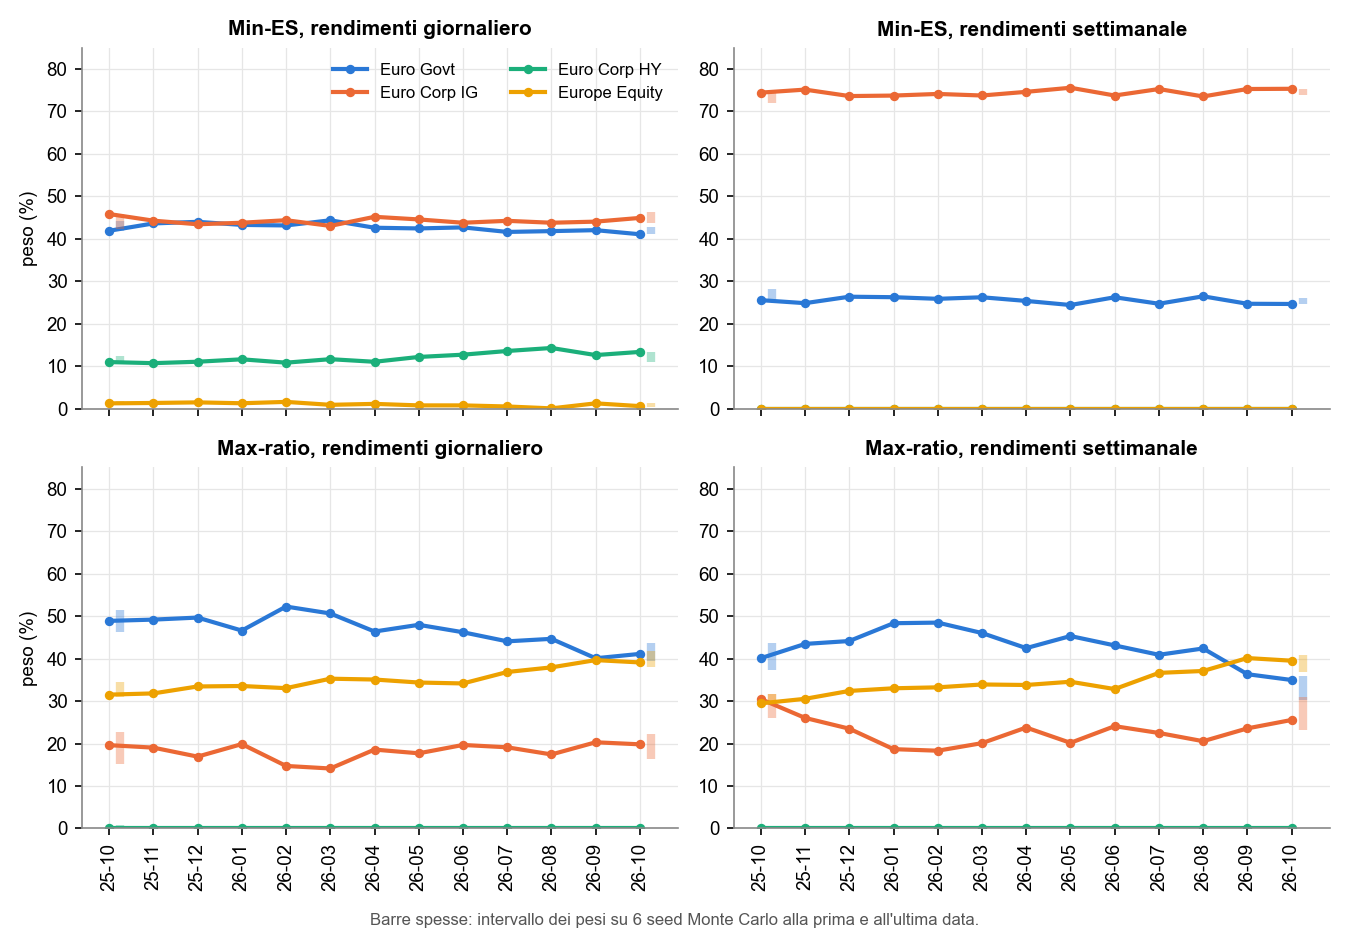
\includegraphics[width=\textwidth]{figures_100k/weights}
\caption{Pesi dei due portafogli ottimi a ogni data, 100\,000 scenari. Le barre spesse alla prima e all'ultima data sono l'intervallo dei pesi sui sei seed a dati fissi.}
\label{fig:weights}
\end{figure}

\begin{figure}[htbp]\centering
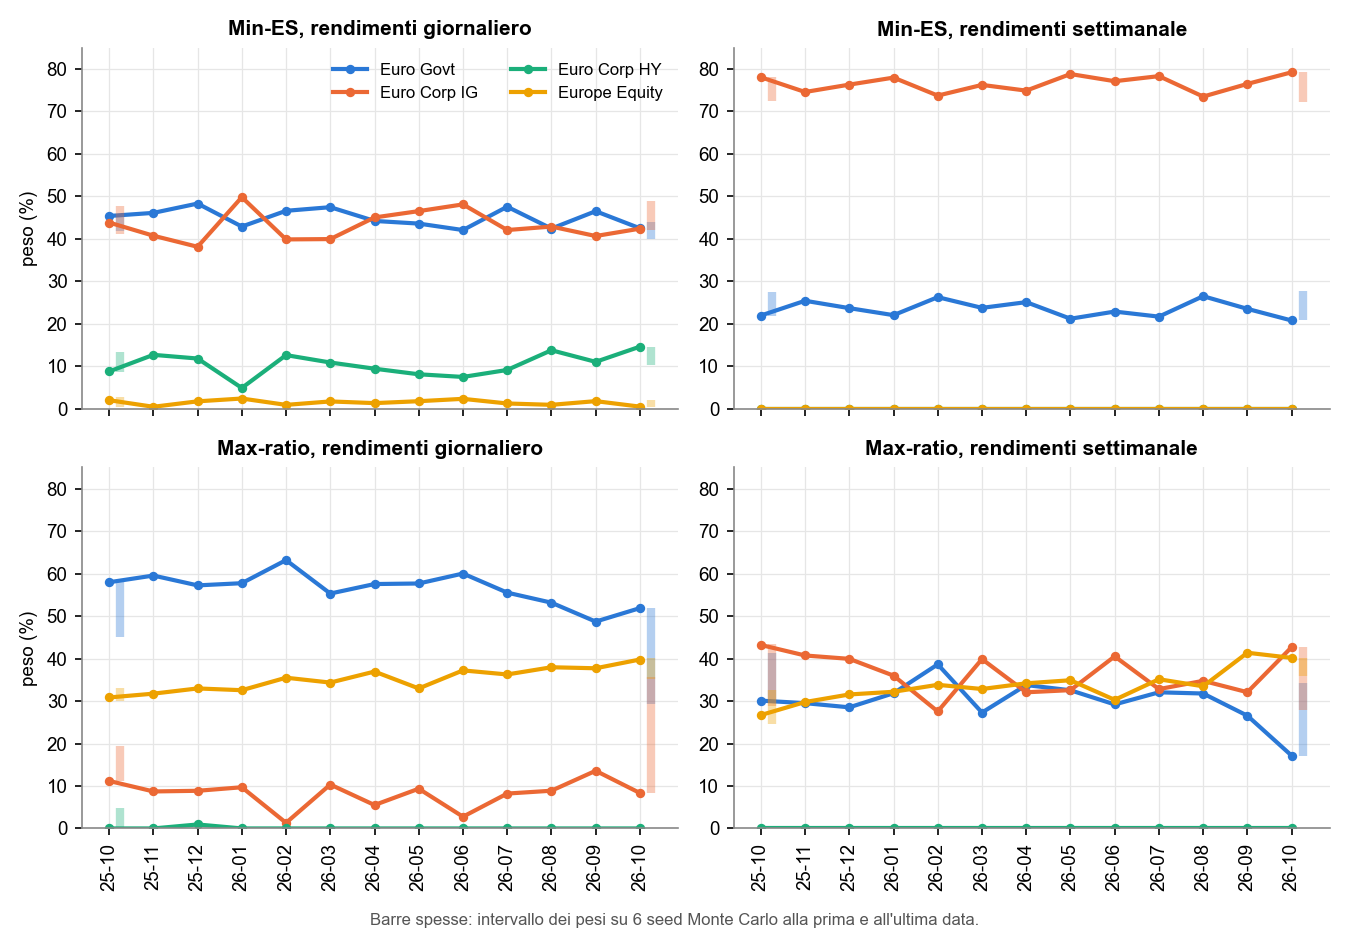
\includegraphics[width=\textwidth]{figures_10k/weights}
\caption{Gli stessi pesi con 10\,000 scenari. Le oscillazioni mensili e le barre del rumore sono della stessa ampiezza: a questo livello i pesi non distinguono i dati dal sorteggio.}
\label{fig:weights_10k}
\end{figure}

\begin{figure}[htbp]\centering
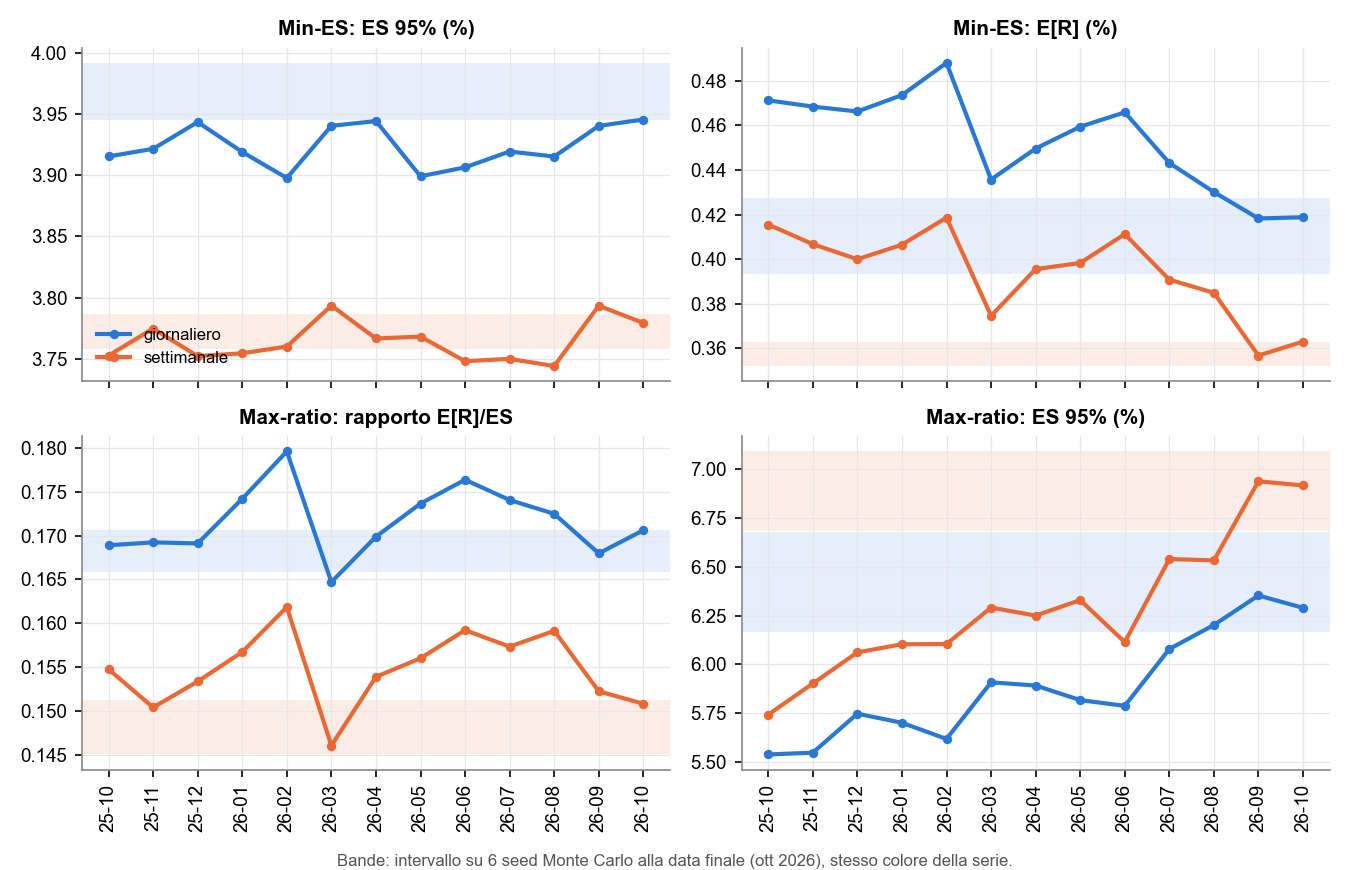
\includegraphics[width=\textwidth]{figures_100k/metrics}
\caption{Metriche dei due portafogli a ogni data, 100\,000 scenari; le bande sono l'intervallo sui sei seed alla data finale.}
\label{fig:metrics}
\end{figure}

\section{Il portafoglio Min-ES}

\subsection{Giornaliero}

L'ES resta fra 3,90\,\% e 3,95\,\%: la sua escursione annua (0,05 punti) coincide con quella sui seed (0,05--0,07). Il rendimento atteso invece ha un andamento chiaro: sale fino a 0,49\,\% a febbraio 2026, scende a 0,44\,\% a marzo e poi gradualmente a 0,42\,\% a ottobre. L'escursione (0,07) \`e il triplo del rumore (0,02--0,03), e segue i dati: il rendimento atteso a 60 giorni dei governativi passa da 0,40\,\% a 0,33\,\% e quello dell'IG da 0,44\,\% a 0,40\,\% (tabella~\ref{tab:runs_daily} e figura~\ref{fig:assets}). A 10\,000 scenari lo stesso calo c'era (0,47 $\to$ 0,41\,\%), ma con un rumore di 0,04 era al limite del rilevabile.

I pesi sono fermi: Govt 41--44\,\%, IG 43--46\,\%, HY 11--14\,\%, azionario 0--1,6\,\%, con escursioni annue (3,3, 2,8, 3,6 e 1,5 punti) poco sopra quelle sui seed (1,8--2,2, 2,6--3,5, 1,4--2,3 e 0,5--0,8). L'unico movimento con una direzione \`e la lenta crescita dell'HY da 11\,\% a 14\,\% fra maggio e agosto 2026, quando l'ES dell'HY scende da 6,57\,\% a 6,47\,\%, e la contemporanea discesa dell'azionario sotto l'1\,\%. Il costo di non aggiornare i pesi (tabella~\ref{tab:cross}) non supera 0,002 punti di ES sul mese successivo e 0,004 sugli scenari finali: tutti i tredici vettori di pesi sono equivalenti entro il rumore.

Con 10\,000 scenari il quadro era diverso (figura~\ref{fig:weights_10k}): Govt 42--48\,\%, IG 38--50\,\%, HY 5--15\,\%, e fra gennaio e febbraio 2026 un salto dell'IG da 49,8\,\% a 39,9\,\% e dell'HY da 4,9\,\% a 12,6\,\%, in un mese di dati tranquilli. Con 100\,000 scenari l'IG passa da 43,8\,\% a 44,4\,\% e l'HY da 11,6\,\% a 10,9\,\%: quel salto era rumore Monte Carlo. La ragione \`e nella figura~\ref{fig:segment}: lungo il segmento Govt/IG l'ES ha un minimo largo, con 4 centesimi di punto di differenza fra 20\,\% e 50\,\% di Govt, e un errore di stima dell'ES di 0,1 punti (quello di 10\,000 scenari) basta a spostare l'argmin di dieci punti. Con un errore di 0,03--0,05 punti l'argmin si sposta di due o tre.

\begin{figure}[htbp]\centering
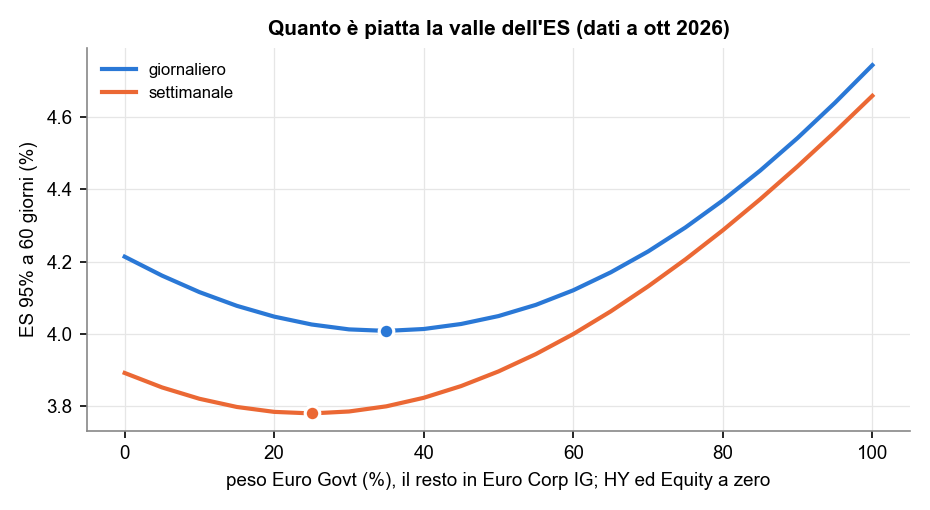
\includegraphics[width=0.75\textwidth]{figures_100k/segment}
\caption{ES a 60 giorni dei portafogli composti solo da Govt e IG, dati a ottobre 2026, 100\,000 scenari. Il minimo \`e una valle: fra 20\,\% e 50\,\% di Govt l'ES giornaliero varia di 0,04 punti.}
\label{fig:segment}
\end{figure}

\subsection{Settimanale}

Il Min-ES settimanale \`e il risultato pi\`u stabile dello studio: ES 3,74--3,79\,\% (escursione 0,05, rumore 0,03--0,08), Govt 24--27\,\% e IG 73--76\,\% (escursione 2 punti, rumore 1--3), HY e azionario a zero in tutti i tredici run e in tutti i dodici run con seed diversi, a entrambi i livelli di scenari. I vincoli di non negativit\`a sono attivi su due asset, il che toglie due gradi di libert\`a all'ottimo e lo irrigidisce. La valle resta piatta anche qui (ES fra 3,78\,\% e 3,82\,\% per Govt fra 10\,\% e 40\,\%), e il costo di non aggiornare i pesi non supera 0,001 punti.

Il rendimento atteso scende da 0,42\,\% a 0,36\,\% (rumore 0,01): lo stesso calo dei governativi visto nel giornaliero, con i due gradini di marzo e di settembre 2026 (settembre: $-2{,}1\,\%$ per il Govt con quattro giorni in coda; tabella~\ref{tab:added}).

\section{Il portafoglio Max-ratio}

\subsection{Il rapporto \`e stabile, l'ES cresce}

Giornaliero: rapporto 0,165--0,180, escursione 0,015 contro 0,005 di rumore. Settimanale: 0,146--0,162, escursione 0,016 contro 0,006--0,009. Il movimento \`e quindi in parte reale, ma non \`e un trend: nelle due frequenze il rapporto sale fino a febbraio 2026, crolla a marzo, risale fino a giugno e cala di nuovo a settembre, e a ottobre 2026 (0,171 e 0,151) \`e vicino a dove era a ottobre 2025 (0,169 e 0,155). La qualit\`a del miglior portafoglio non \`e cambiata nell'anno; \`e cambiato il portafoglio. A 10\,000 scenari il profilo era lo stesso, ma con un rumore di 0,013--0,016 non si distingueva dall'escursione (0,013--0,018).

L'ES del Max-ratio infatti sale in modo netto: da 5,54\,\% a 6,29\,\% nel giornaliero (escursione 0,81, rumore 0,4--0,5) e da 5,74\,\% a 6,92\,\% nel settimanale (1,19 contro 0,3--0,4), con i due gradini di marzo e di luglio--settembre 2026 (figura~\ref{fig:metrics}). Il rendimento atteso sale in parallelo (0,94 $\to$ 1,07\,\% e 0,89 $\to$ 1,04\,\%). Il portafoglio a rapporto massimo si \`e spostato lungo la frontiera verso un punto pi\`u rischioso e pi\`u redditizio, a rapporto quasi invariato.

\subsection{Il peso azionario cresce, i governativi calano: un cambiamento genuino}

Il peso dell'azionario nel Max-ratio sale da 31,5\,\% a 39,1\,\% nel giornaliero (escursione 8,1 punti, rumore 3,5--3,9) e da 29,5\,\% a 39,5\,\% nel settimanale (10,7 contro 2,3--4,0), con un andamento quasi monotono (figura~\ref{fig:weights}). Lo specchio \`e il peso dei governativi: da 48,9\,\% (52,2\,\% a febbraio) a 41,1\,\% nel giornaliero e da 40,1\,\% (48,5\,\% a febbraio) a 35,0\,\% nel settimanale, con escursioni di 12--13 punti contro 4--6 di rumore. L'IG \`e fermo (giornaliero 14--20\,\%, settimanale 18--31\,\%, rumore 6--8). Sono gli unici pesi con un trend chiaro sopra il rumore, e hanno una spiegazione nei dati (figura~\ref{fig:assets}, tabella~\ref{tab:added}):

\begin{itemize}
\item il rendimento atteso a 60 giorni dell'azionario passa da 2,08\,\% a 2,19\,\% (giornaliero), per i mesi forti da novembre 2025 a febbraio 2026 ($+0{,}8$, $+2{,}7$, $+3{,}3$, $+3{,}9\,\%$) e da aprile a giugno 2026 ($+5{,}4$, $+3{,}1$, $+2{,}8\,\%$), mentre il suo ES scende da 14,5\,\% a 14,1\,\%;
\item il rendimento atteso dei governativi scende da 0,40\,\% a 0,33\,\% e il loro ES non migliora (4,72 $\to$ 4,74\,\%), per i tre mesi negativi del 2026 (marzo $-2{,}7\,\%$, luglio $-1{,}8\,\%$, settembre $-2{,}1\,\%$).
\end{itemize}

Un rendimento azionario migliore a parit\`a di coda, contro governativi con meno rendimento e la stessa coda, sposta il massimo del rapporto verso l'azionario. L'ES complessivo cresce perch\'e l'azionario \`e l'asset con la coda pi\`u pesante. Il trend dell'azionario era visibile anche a 10\,000 scenari (31 $\to$ 40\,\% e 27 $\to$ 40\,\%); quello dei governativi no, perch\'e sepolto dal rumore sulla ripartizione Govt/IG.

\begin{figure}[htbp]\centering
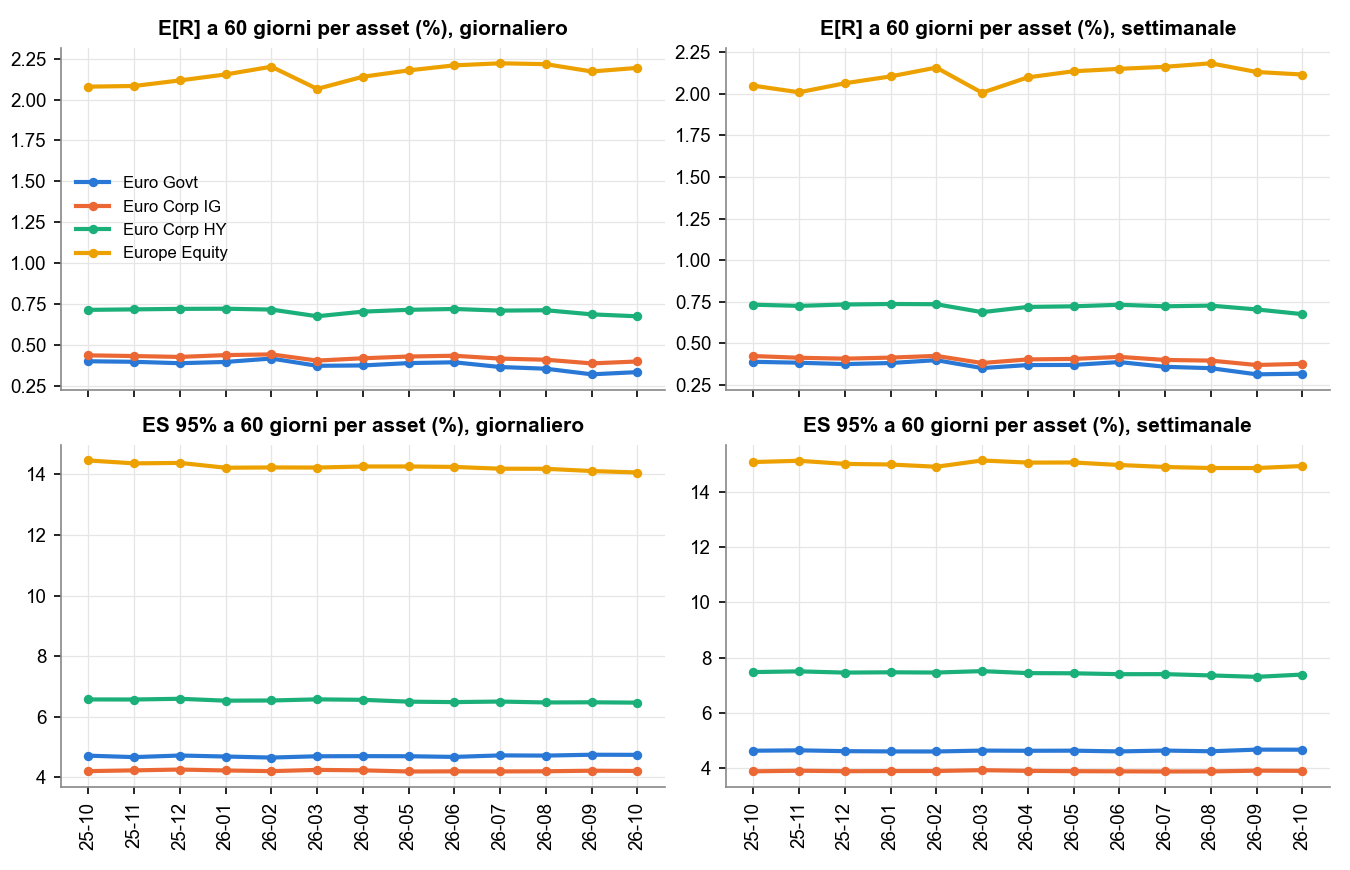
\includegraphics[width=\textwidth]{figures_100k/assets}
\caption{Rendimento atteso ed ES a 60 giorni di ciascun asset a ogni data, 100\,000 scenari: la materia prima delle ottimizzazioni.}
\label{fig:assets}
\end{figure}

\subsection{Govt contro IG: determinato, entro 5--8 punti}

Con 10\,000 scenari la ripartizione della parte obbligazionaria del Max-ratio fra Govt e IG era indeterminata: l'escursione sui seed (23 e 27 punti nel giornaliero) superava quella nell'anno, e il run con seed 42 dava IG fra 1\,\% e 14\,\% (figura~\ref{fig:weights_10k}). Con 100\,000 scenari l'escursione sui seed scende a 4--8 punti in entrambe le frequenze, e i sei seed alla data finale concordano su Govt 39--44\,\% e IG 16--22\,\% (giornaliero), Govt 30--36\,\% e IG 23--31\,\% (settimanale). La ripartizione \`e quindi determinata, con un'incertezza di qualche punto, e la lettura cambia: i livelli di IG del run a 10\,000 scenari (1--14\,\% nel giornaliero) erano un'estrazione sfortunata, non una propriet\`a dei dati. Ci\`o che resta vero \`e che la somma Govt+IG \`e la grandezza meglio determinata (giornaliero 60--69\,\%, settimanale 60--71\,\%, in calo nell'anno come specchio dell'azionario).

\subsection{Marzo 2026}

\`E il solo mese in cui una metrica si muove in un colpo solo di tre volte il rumore: il rapporto giornaliero scende da 0,180 a 0,165 ($-0{,}015$) e quello settimanale da 0,162 a 0,146 ($-0{,}016$). Marzo 2026 ha aggiunto 22 giorni con tutti e quattro gli asset in perdita (Govt $-2{,}7\,\%$, IG $-2{,}3\,\%$, HY $-2{,}4\,\%$, azionario $-7{,}7\,\%$ con un giorno a $-3{,}0\,\%$) e fra 4 e 7 giorni per asset sotto il 5\textsuperscript{o} percentile storico, cio\`e il 2--4\,\% in pi\`u di osservazioni in coda in un mese. Il rendimento atteso di tutti gli asset cala e l'ES sale (figura~\ref{fig:assets}), e il rapporto segue. Nei mesi successivi il rapporto risale, perch\'e aprile--giugno 2026 aggiungono mesi positivi che diluiscono la coda. Febbraio 2026 era il massimo dell'anno dopo quattro mesi consecutivi positivi per l'azionario: parte della discesa \`e ritorno verso la media.

\subsection{Settembre--ottobre 2026}

Settembre aggiunge un altro mese con tutti gli asset negativi (Govt $-2{,}1\,\%$, quattro giorni in coda). Il rapporto scende di 0,005 (giornaliero) e 0,007 (settimanale), cio\`e di circa un rumore; l'ES del Max-ratio tocca il massimo dell'anno (6,35\,\% e 6,94\,\%) e il peso azionario anche (39,6\,\% e 40,1\,\%), con il Govt al minimo (40,1\,\% e 36,3\,\%). Ottobre, positivo per Govt e IG, non cambia nulla oltre il rumore. Settembre non \`e un evento isolato come marzo: \`e l'ultimo passo del trend descritto sopra, il mese in cui i governativi perdono per la terza volta nell'anno.

\section{Giornaliero contro settimanale}

Le due frequenze danno metriche vicine (ES del Min-ES 3,95\,\% contro 3,78\,\%, rapporto del Max-ratio 0,171 contro 0,151 a ottobre 2026) ma pesi sistematicamente diversi. La ragione \`e nelle statistiche dei singoli asset (tabella~\ref{tab:assets}): passando da giornaliero a settimanale la deviazione standard a 60 giorni dell'IG scende del 7\,\% (da 2,02 a 1,88) e quella dell'HY sale del 7\,\% (da 3,14 a 3,36), mentre Govt e azionario scendono del 4\,\%. Due punti del campione settimanale in meno (12 settimane coprono circa 58 giorni) spiegano solo un $-1{,}7\,\%$; il resto \`e dipendenza seriale dentro la settimana, che il bootstrap giornaliero ignora e quello settimanale conserva: ritorno verso la media per l'IG, persistenza per l'HY, tipica di un mercato meno liquido in cui i prezzi degli ETF si aggiustano con ritardo. Inoltre le correlazioni con l'azionario salgono (IG--Equity da 0,28 a 0,42, HY--Equity da 0,62 a 0,70; tabella~\ref{tab:corr}), perch\'e la settimana assorbe le chiusure asincrone dei quattro fondi.

Nel settimanale l'IG \`e quindi un asset pi\`u sicuro e l'HY un asset pi\`u rischioso e meno diversificante. Ne segue tutto il resto: il Min-ES settimanale esclude l'HY e concentra sull'IG; il Max-ratio settimanale tiene 18--31\,\% di IG invece di 14--20\,\%, e un po' meno Govt. Queste differenze sono strutturali e stabili nel tempo (compaiono in tutti i tredici run e in tutti i seed, a entrambi i livelli di scenari), non rumore.

\section{Rendimenti realizzati}

Per i dieci run con 60 giorni di borsa successivi disponibili (ottobre 2025 -- luglio 2026), la figura~\ref{fig:realised} confronta il rendimento che ogni portafoglio ha poi realizzato con il rendimento atteso e con l'ES del run. Il Min-ES ha realizzato fra $-2{,}5\,\%$ e $+2{,}4\,\%$ contro un ES di 3,7--3,9\,\%; il Max-ratio fra $-1{,}9\,\%$ e $+5{,}0\,\%$ contro un ES di 5,5--6,5\,\%. Nessuna finestra ha superato l'ES; la peggiore (giugno 2026, $-2{,}5\,\%$ per il Min-ES) \`e arrivata a due terzi dell'ES. Sono dieci finestre sovrapposte in un anno: una verifica di plausibilit\`a, non un test statistico. Il risultato \`e identico a 10\,000 scenari, perch\'e i pesi dei due livelli differiscono di pochi punti e i rendimenti realizzati sono dati, non simulazioni.

\begin{figure}[htbp]\centering
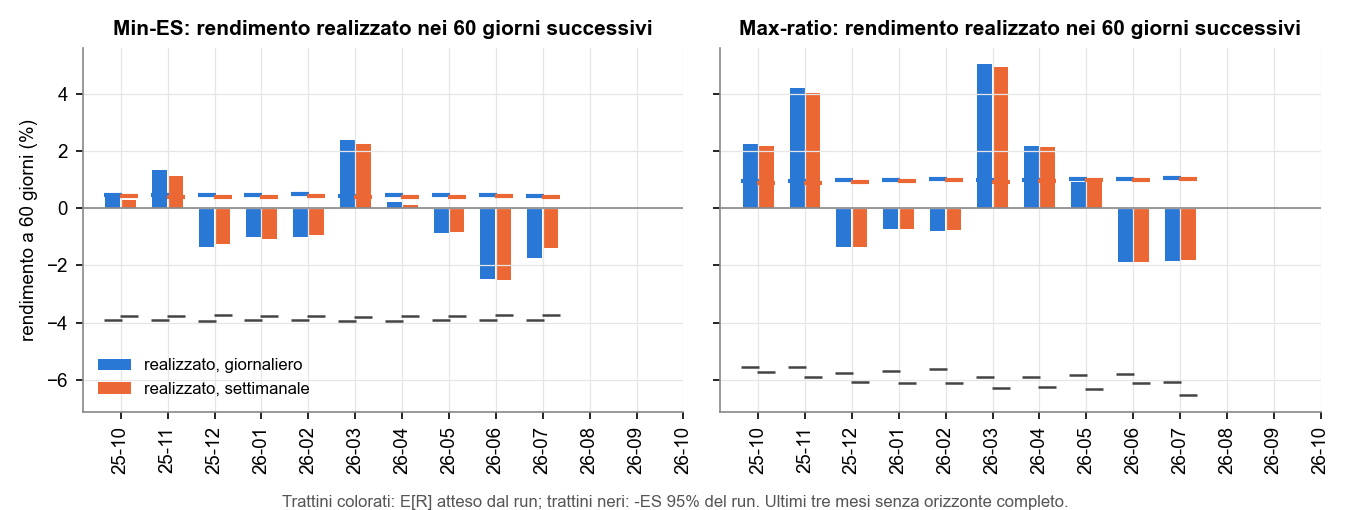
\includegraphics[width=\textwidth]{figures_100k/realised}
\caption{Rendimento realizzato nei 60 giorni di borsa successivi a ogni data, contro rendimento atteso ed ES del run (100\,000 scenari).}
\label{fig:realised}
\end{figure}

\section{Cosa cambia fra 10\,000 e 100\,000 scenari}
\label{sec:cmp}

\begin{table}[htbp]\centering\small\setlength{\tabcolsep}{3.5pt}
\caption{Rumore Monte Carlo: escursione su 6 seed a dati fissi (30 ott 2026) con 10\,000 e con 100\,000 scenari. Metriche in \%, pesi in punti percentuali.}\label{tab:noise_cmp}
\begin{tabular}{lrrrr}\toprule
grandezza & \multicolumn{2}{c}{giornaliero} & \multicolumn{2}{c}{settimanale} \\
 & 10k & 100k & 10k & 100k \\ \midrule
Min-ES: ES 95\,\% & 0.14 & 0.05 & 0.11 & 0.03 \\
Min-ES: E[R] & 0.04 & 0.03 & 0.03 & 0.01 \\
Max-ratio: rapporto & 0.016 & 0.005 & 0.006 & 0.006 \\
Max-ratio: ES 95\,\% & 0.48 & 0.51 & 0.60 & 0.41 \\
Min-ES: peso Govt & 4.1 & 1.8 & 7.0 & 1.4 \\
Min-ES: peso IG & 6.8 & 2.6 & 7.0 & 1.4 \\
Min-ES: peso HY & 4.3 & 2.3 & 0.0 & 0.0 \\
Min-ES: peso Equity & 1.5 & 0.8 & 0.0 & 0.0 \\
Max-ratio: peso Govt & 22.6 & 4.2 & 17.0 & 5.8 \\
Max-ratio: peso IG & 27.3 & 6.1 & 14.8 & 7.9 \\
Max-ratio: peso HY & 0.0 & 0.0 & 0.0 & 0.0 \\
Max-ratio: peso Equity & 5.0 & 3.9 & 4.4 & 4.0 \\
\bottomrule\end{tabular}\end{table}

\begin{table}[htbp]\centering\footnotesize\setlength{\tabcolsep}{4pt}
\caption{Tempi di calcolo (secondi, minimo di due ripetizioni) al variare del numero di scenari; dati a ott 2026, rendimenti giornalieri. LP del notebook = simulazione + due LP + 20 punti di frontiera, senza nuvola casuale e grafici.}\label{tab:bench}
\begin{tabular}{rrrrrrr}\toprule
scenari & simulazione & LP Min-ES & LP Max-ratio & punto frontiera & LP del notebook & scenari (MB) \\ \midrule
10\,000 & 0.08 & 0.6 & 0.8 & 0.6 & 13 & 0.3 \\
25\,000 & 0.23 & 3.2 & 3.7 & 3.6 & 79 & 0.8 \\
50\,000 & 0.70 & 14.4 & 15.4 & 17.0 & 371 & 1.5 \\
100\,000 & 1.42 & 51.8 & 61.5 & 53.8 & 1190 & 3.1 \\
\bottomrule\end{tabular}\end{table}


\paragraph{Rumore.} La tabella~\ref{tab:noise_cmp} confronta l'escursione sui sei seed a dati fissi ai due livelli. L'attesa teorica \`e una riduzione di $\sqrt{10} \approx 3{,}2$. Per le grandezze ben determinate si osserva: ES del Min-ES da 0,14 a 0,05 (giornaliero) e da 0,11 a 0,03 (settimanale), pesi del Min-ES da 4--7 punti a 1--3, ripartizione Govt/IG del Max-ratio da 23--27 punti a 4--8 (giornaliero) e da 15--17 a 6--8 (settimanale), rapporto giornaliero da 0,016 a 0,005. Due grandezze non migliorano: l'ES del Max-ratio (0,5 punti in entrambi i casi nel giornaliero) e il suo peso azionario (5 punti contro 4). Sono le coordinate del punto di massimo lungo la frontiera, e il rapporto \`e piatto in quella direzione: spostare il portafoglio ottimo di ottobre 2026 di 4 punti di azionario (presi dal Govt) cambia il rapporto di 0,0002--0,0004 e l'ES di 0,45 punti, quindi l'argmax resta sensibile al sorteggio anche quando il valore del massimo non lo \`e pi\`u. In pratica: a 100\,000 scenari l'ES del Max-ratio va letto con $\pm 0{,}25$ punti e il suo peso azionario con $\pm 2$ punti; questa incertezza non si compra con altri scenari, ma con la media su pi\`u seed.

\paragraph{Conclusioni che cambiano.} Tre letture del primo esperimento non reggono al secondo:
\begin{itemize}
\item \emph{``I pesi del Min-ES giornaliero oscillano di 10 punti da un mese all'altro.''} Era rumore: a 100\,000 scenari oscillano di 2--4 punti, quanto cambiando seed.
\item \emph{``La ripartizione Govt/IG del Max-ratio \`e indeterminata.''} \`E determinata entro 4--8 punti; i livelli a 10\,000 scenari (IG 1--14\,\% nel giornaliero) erano un'estrazione sfortunata.
\item \emph{``Il rapporto del Max-ratio e il rendimento atteso del Min-ES si muovono entro il rumore.''} Si muovono di tre volte il rumore, con un profilo spiegato dai dati (picco a febbraio 2026, crollo a marzo, calo da settembre).
\end{itemize}
Le altre conclusioni (trend dell'azionario nel Max-ratio, ES in salita, marzo 2026, struttura giornaliero/settimanale, rendimenti realizzati) erano gi\`a corrette a 10\,000 scenari, perch\'e riguardano grandezze il cui movimento supera anche il rumore maggiore.

\paragraph{Un dettaglio sui livelli.} Il run a 10\,000 scenari con seed 42 dava, a ottobre 2026, un rapporto giornaliero di 0,163; quello a 100\,000 d\`a 0,171. Non \`e un bias del numero di scenari: la media sui sei seed \`e 0,169 in entrambi i casi. Il seed 42 era, a 10\,000 scenari, un'estrazione bassa, e tutti i livelli del primo esperimento ne risentivano (rapporto, pesi Govt/IG). \`E la ragione per cui un singolo run a 10\,000 scenari non va usato per confronti fini fra date o fra frequenze.

\section{Tempi di calcolo}
\label{sec:perf}

\paragraph{Un LP alla volta.} La tabella~\ref{tab:bench} d\`a i tempi dei singoli passi a dati fissi. La simulazione \`e trascurabile e cresce in modo quasi lineare (1,4 secondi a 100\,000 scenari). Gli LP no: ogni scenario aggiunge una variabile ausiliaria e un vincolo alla formulazione di Rockafellar--Uryasev, e il tempo di HiGHS cresce con un esponente di circa 1,9 nel numero di scenari, cio\`e quasi col quadrato. Passare da 10\,000 a 100\,000 scenari moltiplica il tempo di un LP per 75--90: da 0,6--0,8 secondi a 52--62. La memoria non \`e un vincolo: la matrice degli scenari occupa 3 MB a 100\,000 scenari, e il picco di memoria del processo R durante un LP a 100\,000 scenari \`e di 494 MB (misurato campionando il working set).

\paragraph{Lo studio e il notebook.} Lo studio di stabilit\`a esegue 46 run (13 mesi $\times$ 2 frequenze, pi\`u 20 run con seed diversi), ciascuno con due LP: 92 LP in tutto, 66 secondi a 10\,000 scenari e 5\,622 secondi (94 minuti) a 100\,000. Il notebook del progetto esegue un run solo, ma con la frontiera: 2 + 50 LP sulla stessa matrice di scenari (la simulazione non viene ripetuta: ogni punto \`e il LP Min-ES con un vincolo in pi\`u sul rendimento atteso), pi\`u la nuvola di 3\,000 portafogli casuali e i grafici. La tabella~\ref{tab:notebook} riporta i tempi misurati passo per passo.

\begin{table}[htbp]\centering\small
\caption{Tempi misurati del notebook (secondi), stessi passi del file \texttt{Asset Allocation EUR.Rmd}, dati a ottobre 2026. ``Fissi'' = lettura dati, simulazione, statistiche, due grafici con ggplot e loro salvataggio.}\label{tab:notebook}
\begin{tabular}{rrrrrrr}\toprule
scenari & punti frontiera & nuvola & LP Min-ES + Max-ratio & frontiera & fissi & totale \\ \midrule
10\,000 & 50 & 3,7 & 2,8 & 39,0 & 4,5 & 50,7 \\
10\,000 & 20 & 3,4 & 2,5 & 14,4 & 3,1 & 24,0 \\
100\,000 & 50 & 31,7 & 132,2 & 4\,348,7 & 6,2 & 4\,519,9 \\
\bottomrule\end{tabular}
\end{table}

Due cose si leggono dalla tabella. La prima: a 10\,000 scenari il notebook impiega \nbTenFifty{} secondi, di cui 39 nei 50 LP della frontiera, che \`e un elemento illustrativo; i due portafogli ottimi costano meno di 3 secondi. La seconda: a 100\,000 scenari il notebook impiega 75 minuti, di cui 72 nella frontiera (87 secondi per punto: pi\`u dei 54 del punto isolato della tabella~\ref{tab:bench}, perch\'e i vincoli di rendimento vicini al massimo rendono il LP pi\`u difficile) e 32 nella nuvola casuale, mentre i due portafogli ottimi arrivano in poco pi\`u di due minuti. La frontiera \`e una curva liscia e 20 punti la disegnano quanto 50.

\paragraph{Quanti scenari in dieci secondi.} Con 50 punti di frontiera il notebook sta sotto i dieci secondi solo con circa 2\,000 scenari (10,6 secondi misurati), un livello al quale il rumore sarebbe il doppio di quello a 10\,000. Il budget \`e dominato da costi fissi di circa 5 secondi, indipendenti dagli scenari: 1,5 secondi di avvio di HiGHS al primo LP e 3,5 secondi per i due grafici. Dei 5 secondi restanti, a 10\,000 scenari la nuvola di 3\,000 portafogli ne prende 4 (0,4 secondi ogni 1\,000 scenari) e la frontiera a 50 punti 39. Le leve, in ordine di efficacia, sono quindi i punti di frontiera, la dimensione della nuvola e solo per ultimo il numero di scenari: con 10 punti e 1\,000 portafogli nella nuvola si stimano circa 8\,000 scenari in dieci secondi; per i soli portafogli ottimi, senza frontiera n\'e nuvola, 10\,000 scenari costano circa 7 secondi e 15\,000 sono il limite.

\paragraph{Decisione.} A valle dello studio il default del tool \`e stato lasciato a 10\,000 scenari e \texttt{N\_FRONTIER} portato da 50 a 20 (commit del 2 novembre 2026 nel repository, con notebook, README e guida aggiornati): il notebook passa da \nbTenFifty{} a \nbTenTwenty{} secondi. Per confronti fini fra date o fra frequenze, dove i pesi contano, le opzioni sono due: 100\,000 scenari (circa due minuti per i due portafogli ottimi, pi\`u \nbHundredTwenty{} per i 20 punti di frontiera), oppure la media dei pesi su sei seed a 10\,000 scenari, che costa 4 secondi per portafoglio e riduce il rumore di $\sqrt{6} \approx 2{,}4$, circa quanto 50\,000 scenari; la media dei pesi non \`e esattamente un ottimo, ma nella valle piatta la differenza \`e trascurabile (tabella~\ref{tab:cross}), e l'escursione fra i seed \`e di per s\'e un'informazione utile da riportare.

\section{Elenco dei cambiamenti maggiori e loro giustificazione}

\begin{enumerate}
\item \textbf{Peso azionario del Max-ratio da 31,5 a 39\,\% (giornaliero) e da 29,5 a 39,5\,\% (settimanale), governativi da 49 a 41\,\% e da 40 a 35\,\%, ES da 5,5 a 6,3\,\% e da 5,7 a 6,9\,\%.} Genuino (escursioni di 2--3 volte il rumore, andamento monotono): rendimento atteso dell'azionario in salita e governativi con rendimento in calo nel 2026. Il rapporto a fine anno \`e dov'era: il portafoglio migliore \`e diventato pi\`u rischioso, non peggiore.
\item \textbf{Rapporto del Max-ratio in calo di 0,015 (giornaliero) e 0,016 (settimanale) a marzo 2026.} Genuino ma transitorio: correzione simultanea di tutti gli asset, 2--4\,\% di osservazioni in coda in pi\`u; riassorbito da aprile a giugno.
\item \textbf{Rendimento atteso del Min-ES da 0,47 a 0,42\,\% (giornaliero) e da 0,42 a 0,36\,\% (settimanale), con picco a febbraio 2026.} Genuino (tre e sei volte il rumore): tre mesi negativi per i governativi, che sono met\`a (giornaliero) o un quarto (settimanale) del portafoglio.
\item \textbf{Pesi del Min-ES.} Nessun cambiamento maggiore: escursioni di 2--4 punti, dell'ordine del rumore. Il salto di 10 punti fra gennaio e febbraio 2026 visto con 10\,000 scenari era rumore Monte Carlo nella valle piatta dell'ES.
\item \textbf{Ripartizione Govt/IG nel Max-ratio.} Determinata entro 5--8 punti; l'indeterminazione di 15--25 punti vista con 10\,000 scenari era rumore. Il trend dei governativi (punto 1) \`e reale; l'IG \`e fermo.
\item \textbf{Esclusione di HY e azionario dal Min-ES settimanale.} Strutturale: dipende dalla frequenza, non dalla data n\'e dal seed.
\end{enumerate}

\section{Conclusioni e indicazioni d'uso}

\begin{itemize}
\item Il tool \`e stabile: con 100\,000 scenari, ES, rendimento atteso, rapporto e pesi dei portafogli ottimi si muovono nell'anno quanto si muovono cambiando seed, salvo i cambiamenti che i dati giustificano (azionario che guadagna peso sui governativi nel Max-ratio, rendimento atteso in calo nel Min-ES, il mese di marzo 2026).
\item Con 10\,000 scenari, il default del tool, le metriche sono gi\`a affidabili e i cambiamenti grandi si vedono; met\`a delle oscillazioni dei pesi \`e per\`o rumore Monte Carlo, e un singolo run pu\`o essere un'estrazione sfortunata: il run con seed 42 sottostimava il rapporto di 0,006 e l'IG del Max-ratio di circa 10 punti. A quel livello i pesi vanno letti insieme alla forma della superficie, e dove questa \`e piatta (Govt contro IG) il singolo numero \`e un'estrazione da un intervallo.
\item Il costo degli scenari cresce col quadrato; quello della frontiera \`e lineare nei punti ed \`e la voce dominante del notebook. Per questo il default resta 10\,000 scenari con 20 punti di frontiera; per i confronti fini si usano 100\,000 scenari o la media su pi\`u seed.
\item La posizione del Max-ratio lungo la frontiera (ES e peso azionario) resta rumorosa anche a 100\,000 scenari, perch\'e il rapporto \`e piatto attorno al massimo: va riportata con un intervallo ($\pm 0{,}25$ punti di ES, $\pm 2$ punti di azionario).
\item La scelta della frequenza non \`e neutra: il settimanale conserva la dipendenza dentro la settimana e penalizza l'HY, il giornaliero ha cinque volte pi\`u punti di supporto. Il Min-ES settimanale \`e il pi\`u stabile dei quattro portafogli; il Max-ratio giornaliero ha il rapporto pi\`u alto. Conviene dichiarare la frequenza insieme ai risultati e, se si confrontano le due, confrontare le metriche e non i pesi.
\end{itemize}

\appendix
\section{Tabelle di dettaglio, 100\,000 scenari}

\begin{table}[htbp]\centering\scriptsize\setlength{\tabcolsep}{3.5pt}
\caption{Run mensili con rendimenti giornaliero, seed 42. $n$ = periodi nel campione; E[R] ed ES in \%, pesi in \%. Run con 100\,000 scenari.}\label{tab:runs_daily}
\begin{tabular}{lrrrrrrrrrrrrrr}\toprule
mese & $n$ & \multicolumn{6}{c}{Min-ES: E[R], ES, pesi Govt/IG/HY/Eq} & \multicolumn{7}{c}{Max-ratio: E[R], ES, rapporto, pesi Govt/IG/HY/Eq} \\\midrule
2025-10 & 3778 & 0.47 & 3.92 & 41.9 & 45.8 & 11.0 & 1.3 & 0.94 & 5.54 & 0.169 & 48.9 & 19.6 & 0.0 & 31.5 \\
2025-11 & 3798 & 0.47 & 3.92 & 43.6 & 44.3 & 10.7 & 1.4 & 0.94 & 5.55 & 0.169 & 49.2 & 19.0 & 0.0 & 31.8 \\
2025-12 & 3817 & 0.47 & 3.94 & 44.0 & 43.4 & 11.1 & 1.5 & 0.97 & 5.75 & 0.169 & 49.7 & 16.9 & 0.0 & 33.4 \\
2026-01 & 3838 & 0.47 & 3.92 & 43.3 & 43.8 & 11.6 & 1.3 & 0.99 & 5.70 & 0.174 & 46.6 & 19.9 & 0.0 & 33.5 \\
2026-02 & 3858 & 0.49 & 3.90 & 43.2 & 44.4 & 10.8 & 1.6 & 1.01 & 5.62 & 0.180 & 52.2 & 14.7 & 0.0 & 33.0 \\
2026-03 & 3880 & 0.44 & 3.94 & 44.4 & 43.0 & 11.7 & 0.9 & 0.97 & 5.91 & 0.165 & 50.6 & 14.1 & 0.0 & 35.3 \\
2026-04 & 3900 & 0.45 & 3.94 & 42.6 & 45.2 & 11.1 & 1.1 & 1.00 & 5.89 & 0.170 & 46.4 & 18.6 & 0.0 & 35.1 \\
2026-05 & 3920 & 0.46 & 3.90 & 42.5 & 44.6 & 12.2 & 0.8 & 1.01 & 5.82 & 0.174 & 47.9 & 17.7 & 0.0 & 34.4 \\
2026-06 & 3942 & 0.47 & 3.91 & 42.7 & 43.8 & 12.7 & 0.8 & 1.02 & 5.79 & 0.176 & 46.2 & 19.7 & 0.0 & 34.1 \\
2026-07 & 3965 & 0.44 & 3.92 & 41.6 & 44.2 & 13.6 & 0.5 & 1.06 & 6.08 & 0.174 & 44.1 & 19.1 & 0.0 & 36.8 \\
2026-08 & 3986 & 0.43 & 3.92 & 41.8 & 43.8 & 14.3 & 0.1 & 1.07 & 6.20 & 0.172 & 44.6 & 17.4 & 0.0 & 37.9 \\
2026-09 & 4008 & 0.42 & 3.94 & 42.0 & 44.1 & 12.6 & 1.3 & 1.07 & 6.35 & 0.168 & 40.1 & 20.3 & 0.0 & 39.6 \\
2026-10 & 4030 & 0.42 & 3.95 & 41.1 & 44.9 & 13.4 & 0.6 & 1.07 & 6.29 & 0.171 & 41.1 & 19.8 & 0.0 & 39.1 \\
\bottomrule\end{tabular}\end{table}

\begin{table}[htbp]\centering\scriptsize\setlength{\tabcolsep}{3.5pt}
\caption{Run mensili con rendimenti settimanale, seed 42. $n$ = periodi nel campione; E[R] ed ES in \%, pesi in \%. Run con 100\,000 scenari.}\label{tab:runs_weekly}
\begin{tabular}{lrrrrrrrrrrrrrr}\toprule
mese & $n$ & \multicolumn{6}{c}{Min-ES: E[R], ES, pesi Govt/IG/HY/Eq} & \multicolumn{7}{c}{Max-ratio: E[R], ES, rapporto, pesi Govt/IG/HY/Eq} \\\midrule
2025-10 & 775 & 0.42 & 3.75 & 25.6 & 74.4 & 0.0 & 0.0 & 0.89 & 5.74 & 0.155 & 40.1 & 30.5 & 0.0 & 29.5 \\
2025-11 & 779 & 0.41 & 3.77 & 24.9 & 75.1 & 0.0 & 0.0 & 0.89 & 5.90 & 0.150 & 43.4 & 26.0 & 0.0 & 30.5 \\
2025-12 & 784 & 0.40 & 3.75 & 26.4 & 73.6 & 0.0 & 0.0 & 0.93 & 6.06 & 0.153 & 44.1 & 23.5 & 0.0 & 32.4 \\
2026-01 & 788 & 0.41 & 3.75 & 26.3 & 73.7 & 0.0 & 0.0 & 0.96 & 6.10 & 0.157 & 48.3 & 18.7 & 0.0 & 33.0 \\
2026-02 & 792 & 0.42 & 3.76 & 25.9 & 74.1 & 0.0 & 0.0 & 0.99 & 6.10 & 0.162 & 48.5 & 18.3 & 0.0 & 33.2 \\
2026-03 & 797 & 0.37 & 3.79 & 26.2 & 73.8 & 0.0 & 0.0 & 0.92 & 6.29 & 0.146 & 46.0 & 20.1 & 0.0 & 33.9 \\
2026-04 & 801 & 0.40 & 3.77 & 25.4 & 74.6 & 0.0 & 0.0 & 0.96 & 6.25 & 0.154 & 42.5 & 23.8 & 0.0 & 33.8 \\
2026-05 & 805 & 0.40 & 3.77 & 24.4 & 75.6 & 0.0 & 0.0 & 0.99 & 6.33 & 0.156 & 45.3 & 20.2 & 0.0 & 34.5 \\
2026-06 & 810 & 0.41 & 3.75 & 26.2 & 73.8 & 0.0 & 0.0 & 0.97 & 6.11 & 0.159 & 43.1 & 24.1 & 0.0 & 32.8 \\
2026-07 & 814 & 0.39 & 3.75 & 24.7 & 75.3 & 0.0 & 0.0 & 1.03 & 6.54 & 0.157 & 40.9 & 22.5 & 0.0 & 36.6 \\
2026-08 & 819 & 0.38 & 3.74 & 26.5 & 73.5 & 0.0 & 0.0 & 1.04 & 6.53 & 0.159 & 42.4 & 20.5 & 0.0 & 37.1 \\
2026-09 & 823 & 0.36 & 3.79 & 24.7 & 75.3 & 0.0 & 0.0 & 1.06 & 6.94 & 0.152 & 36.3 & 23.6 & 0.0 & 40.1 \\
2026-10 & 827 & 0.36 & 3.78 & 24.7 & 75.3 & 0.0 & 0.0 & 1.04 & 6.92 & 0.151 & 35.0 & 25.5 & 0.0 & 39.5 \\
\bottomrule\end{tabular}\end{table}

\begin{table}[htbp]\centering\footnotesize\setlength{\tabcolsep}{3.5pt}
\caption{Stessi dati (fino al 30 ott 2026), sei seed del bootstrap: la variabilit\`a dovuta al solo campionamento Monte Carlo. Run con 100\,000 scenari.}\label{tab:seeds}
\begin{tabular}{lrrlrrl}\toprule
freq. & seed & Min-ES: ES & pesi & Max-ratio: rapporto & ES & pesi \\\midrule
giornaliero & 1 & 3.96 & 42.8/44.8/12.0/0.5 & 0.166 & 6.68 & 39.4/18.7/0.0/41.9 \\
giornaliero & 2 & 3.97 & 42.0/45.0/11.8/1.2 & 0.169 & 6.22 & 42.4/19.6/0.0/38.0 \\
giornaliero & 3 & 3.99 & 42.9/43.8/12.5/0.8 & 0.167 & 6.58 & 42.3/16.3/0.0/41.4 \\
giornaliero & 4 & 3.95 & 42.4/44.5/11.9/1.3 & 0.169 & 6.17 & 39.6/22.3/0.0/38.1 \\
giornaliero & 5 & 3.96 & 41.4/46.4/11.1/1.2 & 0.171 & 6.40 & 43.7/16.3/0.0/40.0 \\
giornaliero & 42 & 3.95 & 41.1/44.9/13.4/0.6 & 0.171 & 6.29 & 41.1/19.8/0.0/39.1 \\
settimanale & 1 & 3.76 & 25.5/74.5/0.0/0.0 & 0.149 & 6.81 & 30.2/31.0/0.0/38.8 \\
settimanale & 2 & 3.79 & 25.2/74.8/0.0/0.0 & 0.151 & 7.09 & 36.0/23.1/0.0/40.9 \\
settimanale & 3 & 3.79 & 26.0/74.0/0.0/0.0 & 0.151 & 6.80 & 35.2/25.8/0.0/39.0 \\
settimanale & 4 & 3.77 & 25.4/74.6/0.0/0.0 & 0.145 & 6.68 & 32.1/31.0/0.0/36.9 \\
settimanale & 5 & 3.76 & 25.4/74.6/0.0/0.0 & 0.149 & 6.73 & 31.5/30.7/0.0/37.8 \\
settimanale & 42 & 3.78 & 24.7/75.3/0.0/0.0 & 0.151 & 6.92 & 35.0/25.5/0.0/39.5 \\
\bottomrule\end{tabular}\end{table}

\begin{table}[htbp]\centering\footnotesize\setlength{\tabcolsep}{3.5pt}
\caption{Costo di usare i pesi di un mese sugli scenari del mese successivo e sugli scenari finali (ott 2026): differenza fra la metrica dei pesi ``vecchi'' e l'ottimo di quel mese. ES in punti percentuali, rapporto in valore assoluto. Run con 100\,000 scenari.}\label{tab:cross}
\begin{tabular}{llrrrr}\toprule
freq. & pesi del mese & $\Delta$ES, mese dopo & $\Delta$rapp., mese dopo & $\Delta$ES, finale & $\Delta$rapp., finale \\\midrule
giornaliero & 2025-10 & +0.001 & -0.0000 & +0.002 & -0.0016 \\
giornaliero & 2025-11 & +0.000 & -0.0001 & +0.003 & -0.0015 \\
giornaliero & 2025-12 & +0.000 & -0.0000 & +0.004 & -0.0010 \\
giornaliero & 2026-01 & +0.000 & -0.0002 & +0.002 & -0.0008 \\
giornaliero & 2026-02 & +0.001 & -0.0001 & +0.003 & -0.0013 \\
giornaliero & 2026-03 & +0.001 & -0.0001 & +0.003 & -0.0007 \\
giornaliero & 2026-04 & +0.000 & -0.0000 & +0.002 & -0.0005 \\
giornaliero & 2026-05 & +0.000 & -0.0000 & +0.001 & -0.0007 \\
giornaliero & 2026-06 & +0.000 & -0.0002 & +0.001 & -0.0006 \\
giornaliero & 2026-07 & +0.000 & -0.0000 & +0.000 & -0.0001 \\
giornaliero & 2026-08 & +0.002 & -0.0001 & +0.001 & -0.0001 \\
giornaliero & 2026-09 & +0.001 & -0.0000 & +0.001 & -0.0000 \\
giornaliero & 2026-10 & -- & -- & +0.000 & +0.0000 \\
settimanale & 2025-10 & +0.000 & -0.0000 & +0.000 & -0.0016 \\
settimanale & 2025-11 & +0.000 & -0.0001 & +0.000 & -0.0015 \\
settimanale & 2025-12 & +0.000 & -0.0000 & +0.001 & -0.0010 \\
settimanale & 2026-01 & +0.000 & -0.0000 & +0.000 & -0.0012 \\
settimanale & 2026-02 & +0.000 & -0.0000 & +0.000 & -0.0012 \\
settimanale & 2026-03 & +0.000 & -0.0000 & +0.000 & -0.0008 \\
settimanale & 2026-04 & +0.000 & -0.0000 & +0.000 & -0.0007 \\
settimanale & 2026-05 & +0.001 & -0.0000 & +0.000 & -0.0007 \\
settimanale & 2026-06 & +0.000 & -0.0002 & +0.000 & -0.0009 \\
settimanale & 2026-07 & +0.001 & -0.0000 & +0.000 & -0.0002 \\
settimanale & 2026-08 & +0.001 & -0.0002 & +0.001 & -0.0002 \\
settimanale & 2026-09 & +0.000 & -0.0000 & +0.000 & -0.0000 \\
settimanale & 2026-10 & -- & -- & +0.000 & +0.0000 \\
\bottomrule\end{tabular}\end{table}

\begin{table}[htbp]\centering\scriptsize\setlength{\tabcolsep}{3.5pt}
\caption{Cosa ha aggiunto ogni mese al campione: rendimento del mese per asset (\%), peggior giorno (\%) e numero di giorni sotto il 5\textsuperscript{o} percentile storico dei rendimenti giornalieri (Govt/IG/HY/Equity). Run con 100\,000 scenari.}\label{tab:added}
\begin{tabular}{lrrrrrrrrrl}\toprule
mese & giorni & \multicolumn{4}{c}{rendimento: Govt, IG, HY, Eq} & \multicolumn{4}{c}{peggior giorno} & giorni in coda \\\midrule
2025-11 & 20 & -0.1 & -0.1 & +0.4 & +0.8 & -0.3 & -0.3 & -0.2 & -1.8 & 0/0/0/1 \\
2025-12 & 19 & -0.5 & -0.2 & +0.5 & +2.7 & -0.4 & -0.4 & -0.1 & -0.6 & 0/1/0/0 \\
2026-01 & 21 & +0.5 & +0.8 & +0.3 & +3.3 & -0.5 & -0.2 & -0.2 & -1.3 & 0/0/0/0 \\
2026-02 & 20 & +1.5 & +0.5 & +0.0 & +3.8 & -0.2 & -0.1 & -0.1 & -0.9 & 0/0/0/0 \\
2026-03 & 22 & -2.7 & -2.3 & -2.4 & -7.6 & -0.8 & -0.7 & -0.8 & -3.0 & 5/7/4/4 \\
2026-04 & 20 & +0.3 & +1.0 & +2.0 & +5.4 & -0.8 & -0.6 & -0.3 & -1.0 & 1/2/0/0 \\
2026-05 & 20 & +1.1 & +0.9 & +1.0 & +3.0 & -0.7 & -0.4 & -0.3 & -1.8 & 1/1/0/1 \\
2026-06 & 22 & +0.5 & +0.4 & +0.5 & +2.8 & -0.5 & -0.3 & -0.2 & -0.7 & 0/0/0/0 \\
2026-07 & 23 & -1.8 & -1.0 & -0.4 & +1.2 & -0.7 & -0.5 & -0.4 & -1.6 & 1/1/0/0 \\
2026-08 & 21 & -0.6 & -0.3 & +0.4 & +0.4 & -0.5 & -0.3 & -0.2 & -0.8 & 0/0/0/0 \\
2026-09 & 22 & -2.1 & -1.3 & -1.4 & -2.3 & -0.7 & -0.5 & -0.5 & -1.4 & 4/2/2/0 \\
2026-10 & 22 & +1.1 & +1.0 & -0.6 & +1.9 & -0.5 & -0.3 & -0.4 & -1.3 & 0/0/0/0 \\
\bottomrule\end{tabular}\end{table}

\begin{table}[htbp]\centering\small\setlength{\tabcolsep}{3.5pt}
\caption{Correlazioni dei log-rendimenti a frequenza giornaliera e settimanale, alla prima e all'ultima data. Run con 100\,000 scenari.}\label{tab:corr}
\begin{tabular}{llrrrrrrr}\toprule
freq. & data & $n$ & Govt--IG & Govt--HY & Govt--Eq & IG--HY & IG--Eq & HY--Eq \\\midrule
giornaliero & 2025-10 & 3778 & 0.67 & 0.21 & 0.05 & 0.57 & 0.27 & 0.62 \\
giornaliero & 2026-10 & 4030 & 0.68 & 0.22 & 0.08 & 0.57 & 0.28 & 0.62 \\
settimanale & 2025-10 & 775 & 0.68 & 0.21 & 0.13 & 0.64 & 0.41 & 0.70 \\
settimanale & 2026-10 & 827 & 0.69 & 0.22 & 0.15 & 0.64 & 0.42 & 0.69 \\
\bottomrule\end{tabular}\end{table}

\begin{table}[htbp]\centering\small\setlength{\tabcolsep}{3.5pt}
\caption{Statistiche dei singoli asset all'orizzonte (60 giorni, scenari del run di ott 2026, seed 42), in \%. Run con 100\,000 scenari.}\label{tab:assets}
\begin{tabular}{lrrrrrrrrrrrr}\toprule
freq. & \multicolumn{4}{c}{E[R]: Govt, IG, HY, Eq} & \multicolumn{4}{c}{dev. std} & \multicolumn{4}{c}{ES 95\,\%} \\\midrule
giornaliero & 0.33 & 0.40 & 0.67 & 2.19 & 2.47 & 2.02 & 3.14 & 8.09 & 4.74 & 4.21 & 6.47 & 14.06 \\
settimanale & 0.32 & 0.38 & 0.68 & 2.11 & 2.37 & 1.88 & 3.36 & 7.77 & 4.66 & 3.89 & 7.39 & 14.95 \\
\bottomrule\end{tabular}\end{table}


\end{document}
